% 图 74.7 —— 由 `checks/emit_hand.py` 自动拼出（probe 精测 + prims2 图元分解）
%%
% ⚠ 这是**稿子不是成品**：跑 `checks/checkhand.py 74.7` 看指标 + 看叠合图。
%%
%% ⚠ 待核：
%   · 本图 probe 报出阴影族 3 个 —— **本脚本不生成阴影**（要照原书手写）；prims2 的 strokes 里可能含阴影线，核对时留意别画重
%   · 可疑字形 4 项（空心圈 ⊙ 常被认成字母 o）—— 见文件末
%%
\documentclass[12pt]{standalone}
\usepackage{fontspec}
\setsansfont{Arial}
\newfontfamily\mfallback{DejaVu Sans}
\usepackage{tikz}
\usetikzlibrary{arrows.meta}
\begin{document}
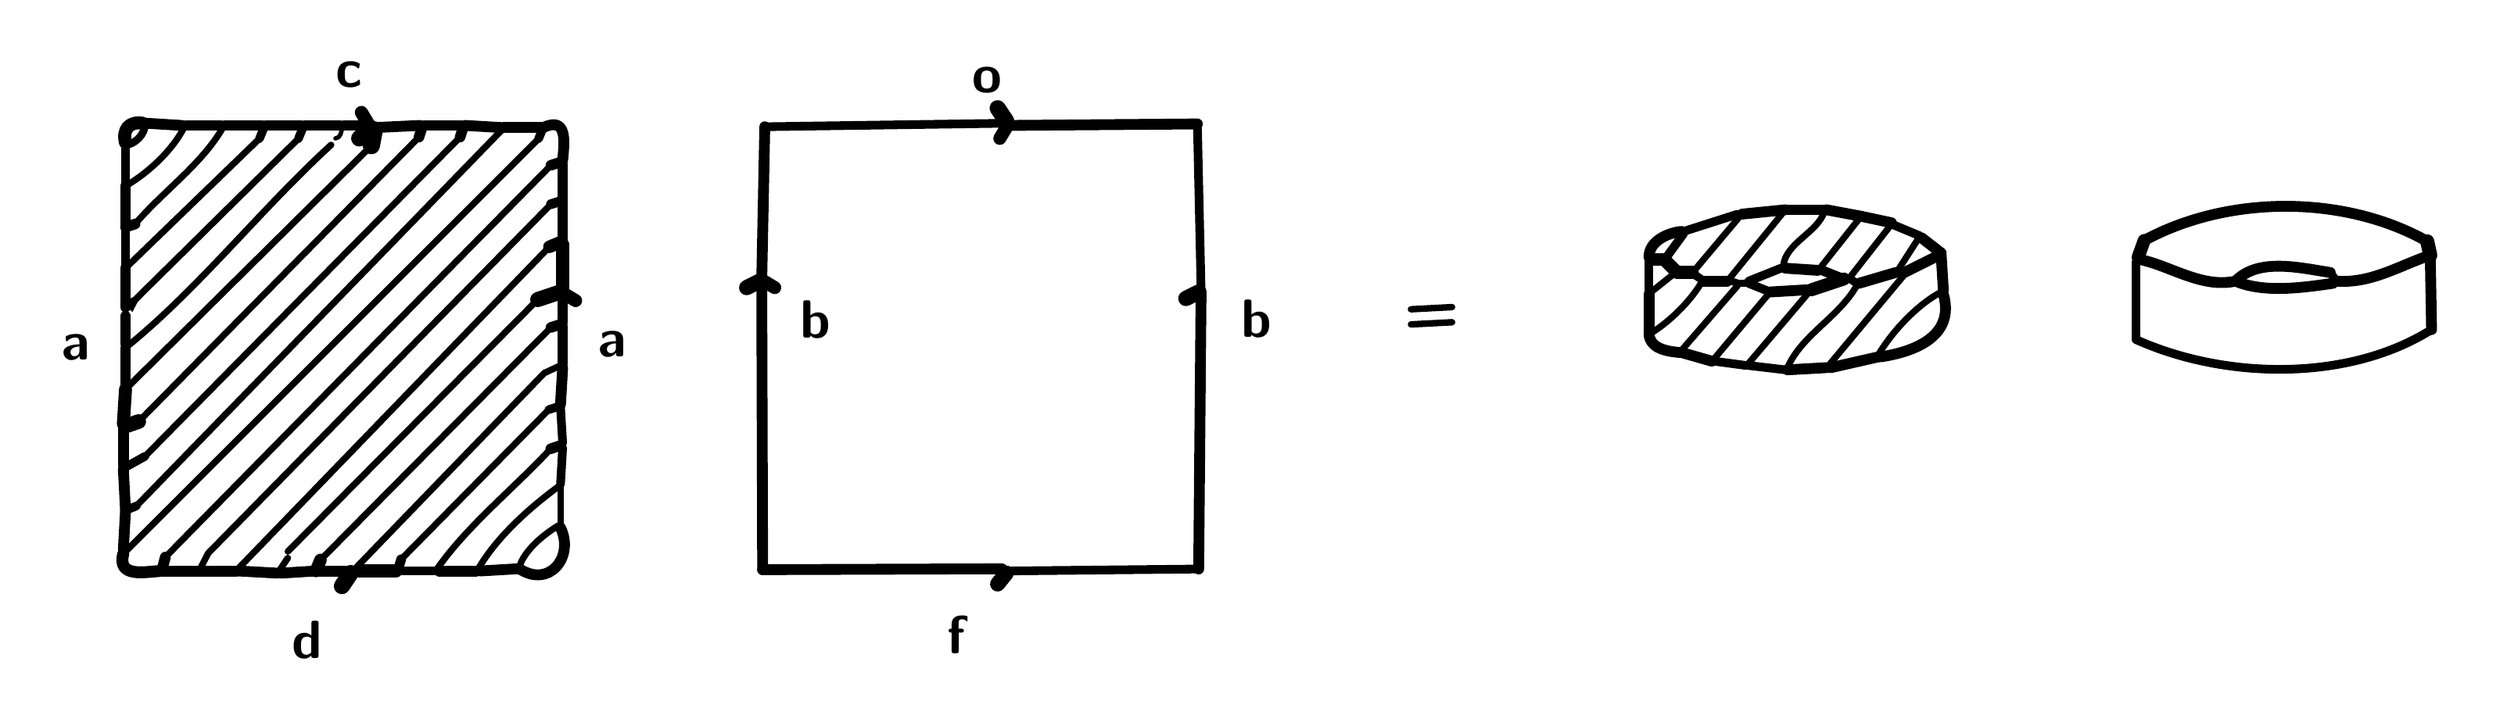
\begin{tikzpicture}[x=1pt, y=-1pt, line width=4.0pt, line cap=round, line join=round]

  %% ════ 直线段（prims2 的 strokes）════
  \draw[line width=4.0pt] (798.0,159.0) -- (815.0,161.0);
  \draw[line width=5.0pt] (48.0,132.0) -- (48.0,114.0);
  \draw[line width=3.0pt] (767.0,152.0) -- (793.0,122.0);
  \draw[line width=4.0pt] (798.0,121.0) -- (808.0,125.0);
  \draw[line width=4.0pt] (877.0,99.0) -- (865.0,94.0);
  \draw[line width=3.0pt] (782.0,156.0) -- (808.0,125.0);
  \draw[line width=5.0pt] (878.0,100.0) -- (887.0,107.0);
  \draw[line width=5.0pt] (184.0,48.0) -- (163.0,49.0);
  \draw[line width=7.5pt] (148.0,261.0) -- (152.0,255.0);
  \draw[line width=5.0pt] (250.0,141.0) -- (250.0,158.0);
  \draw[line width=5.8pt] (136.0,254.0) -- (138.1,248.9);
  \draw[line width=3.0pt] (138.1,248.9) -- (244.6,141.4);
  \draw[line width=4.9pt] (244.6,141.4) -- (249.0,140.0);
  \draw[line width=5.0pt] (136.0,254.0) -- (120.0,255.0);
  \draw[line width=5.0pt] (136.0,254.0) -- (151.0,254.0);
  \draw[line width=5.8pt] (249.0,102.0) -- (243.9,104.1);
  \draw[line width=3.0pt] (243.9,104.1) -- (100.0,253.0);
  \draw[line width=4.0pt] (752.0,111.0) -- (752.0,125.0);
  \draw[line width=4.0pt] (112.0,49.0) -- (109.9,54.1);
  \draw[line width=3.0pt] (109.9,54.1) -- (49.0,113.0);
  \draw[line width=3.4pt] (793.0,121.0) -- (790.0,120.0);
  \draw[line width=4.0pt] (130.0,49.0) -- (127.9,54.1);
  \draw[line width=3.0pt] (127.9,54.1) -- (49.0,132.0);
  \fill (51.2,134.3) -- (46.8,129.7) -- (55.8,125.3) -- cycle;
  \draw[line width=6.0pt] (250.0,103.0) -- (250.0,124.0);
  \draw[line width=3.0pt] (661.0,139.0) -- (642.0,140.0);
  \draw[line width=5.0pt] (47.0,188.0) -- (47.0,205.0);
  \draw[line width=3.0pt] (249.0,159.0) -- (241.5,162.5);
  \draw[line width=3.0pt] (241.5,162.5) -- (155.0,252.0);
  \draw[line width=7.0pt] (335.0,123.0) -- (341.0,120.0);
  \draw[line width=4.0pt] (797.0,159.0) -- (782.0,157.0);
  \draw[line width=4.5pt] (249.0,83.0) -- (244.6,84.4);
  \draw[line width=3.0pt] (244.6,84.4) -- (86.2,245.8);
  \draw[line width=3.0pt] (86.2,245.8) -- (82.0,254.0);
  \draw[line width=5.0pt] (342.0,119.0) -- (343.4,48.6);
  \draw[line width=4.0pt] (343.4,48.6) -- (454.0,47.0);
  \draw[line width=3.0pt] (797.0,121.0) -- (794.0,121.0);
  \draw[line width=4.0pt] (248.0,178.0) -- (243.6,179.4);
  \draw[line width=3.0pt] (243.6,179.4) -- (175.4,248.6);
  \draw[line width=4.5pt] (175.4,248.6) -- (174.0,253.0);
  \draw[line width=3.8pt] (845.0,119.0) -- (848.0,121.0);
  \draw[line width=5.0pt] (147.0,48.0) -- (131.0,48.0);
  \draw[line width=5.0pt] (825.0,124.0) -- (808.0,125.0);
  \draw[line width=5.0pt] (836.0,160.0) -- (858.0,155.0);
  \draw[line width=4.9pt] (52.4,93.6) -- (48.0,95.0);
  \draw[line width=3.0pt] (753.0,125.0) -- (763.0,117.0);
  \draw[line width=5.0pt] (223.0,49.0) -- (241.0,49.0);
  \draw[line width=4.0pt] (241.0,49.0) -- (238.9,54.1);
  \draw[line width=3.0pt] (238.9,54.1) -- (48.0,245.0);
  % （略）线段 (47.0,134.0)-(41.0,137.0) 线宽7.1 —— 是箭头头那一坨，已由箭头头代替
  \draw[line width=5.0pt] (777.0,120.0) -- (788.0,120.0);
  \draw[line width=4.0pt] (48.0,58.0) -- (48.0,76.0);
  \draw[line width=5.0pt] (752.0,144.0) -- (752.0,126.0);
  \draw[line width=6.0pt] (759.0,110.0) -- (753.0,110.0);
  \draw[line width=4.0pt] (48.0,206.0) -- (57.0,201.0);
  \draw[line width=3.0pt] (57.0,201.0) -- (202.6,53.4);
  \draw[line width=4.9pt] (202.6,53.4) -- (204.0,49.0);
  \draw[line width=4.0pt] (793.0,89.0) -- (768.0,97.0);
  \draw[line width=5.0pt] (210.0,254.0) -- (193.0,254.0);
  \draw[line width=5.0pt] (48.0,168.0) -- (48.0,151.0);
  \draw[line width=5.0pt] (250.0,139.0) -- (250.0,127.0);
  \draw[line width=7.4pt] (455.0,46.0) -- (451.0,40.0);
  \draw[line width=5.0pt] (222.0,49.0) -- (205.0,48.0);
  \draw[line width=5.0pt] (250.0,101.0) -- (250.0,83.0);
  \draw[line width=3.8pt] (1066.8,116.0) -- (1069.0,119.0);
  \draw[line width=6.8pt] (48.0,187.0) -- (54.1,184.9);
  \draw[line width=3.0pt] (54.1,184.9) -- (183.6,53.4);
  \draw[line width=4.9pt] (183.6,53.4) -- (185.0,49.0);
  \draw[line width=4.5pt] (48.0,149.0) -- (48.0,136.0);
  \draw[line width=6.0pt] (765.0,116.0) -- (772.0,116.0);
  \draw[line width=6.0pt] (455.0,49.0) -- (452.0,54.0);
  \draw[line width=5.0pt] (47.0,244.0) -- (48.0,226.0);
  \draw[line width=3.0pt] (249.0,215.0) -- (249.0,232.0);
  \draw[line width=3.0pt] (831.0,114.0) -- (850.0,90.0);
  \draw[line width=5.0pt] (250.0,82.0) -- (250.0,66.0);
  \draw[line width=5.0pt] (832.0,87.0) -- (815.0,87.0);
  \draw[line width=5.0pt] (834.0,160.0) -- (816.0,161.0);
  \draw[line width=5.0pt] (249.0,177.0) -- (250.0,160.0);
  \draw[line width=3.0pt] (863.0,95.0) -- (845.0,118.0);
  \draw[line width=4.0pt] (191.0,254.0) -- (175.0,254.0);
  \draw[line width=5.0pt] (113.0,48.0) -- (129.0,48.0);
  \draw[line width=4.0pt] (456.0,254.0) -- (543.9,253.1);
  \draw[line width=5.0pt] (543.9,253.1) -- (545.0,126.0);
  \draw[line width=5.0pt] (65.0,254.0) -- (82.0,254.0);
  \draw[line width=4.9pt] (249.0,196.0) -- (244.5,197.5);
  \draw[line width=7.5pt] (156.0,54.0) -- (161.0,49.0);
  \draw[line width=5.0pt] (886.0,108.0) -- (870.0,116.0);
  \draw[line width=7.9pt] (163.0,50.0) -- (161.6,57.4);
  \draw[line width=3.0pt] (161.6,57.4) -- (49.0,169.0);
  \draw[line width=4.0pt] (48.0,113.0) -- (48.0,95.0);
  \draw[line width=6.0pt] (343.0,120.0) -- (348.0,123.0);
  \draw[line width=5.0pt] (767.0,153.0) -- (781.0,157.0);
  \draw[line width=5.0pt] (76.0,48.0) -- (92.0,48.0);
  \draw[line width=3.0pt] (123.0,245.0) -- (238.5,128.5);
  \draw[line width=7.0pt] (238.5,128.5) -- (249.0,125.0);
  \draw[line width=5.0pt] (94.0,48.0) -- (111.0,48.0);
  \draw[line width=6.0pt] (251.0,126.0) -- (256.0,129.0);
  \draw[line width=5.0pt] (850.0,90.0) -- (834.0,87.0);
  \draw[line width=5.0pt] (850.0,90.0) -- (864.0,93.0);
  \draw[line width=3.0pt] (826.0,125.0) -- (798.0,158.0);
  \draw[line width=5.0pt] (118.0,255.0) -- (100.0,254.0);
  \draw[line width=5.0pt] (48.0,76.0) -- (48.0,95.0);
  \draw[line width=3.0pt] (123.0,248.0) -- (119.0,254.0);
  \draw[line width=5.0pt] (866.0,116.0) -- (849.0,121.0);
  \draw[line width=6.0pt] (760.0,111.0) -- (764.0,115.0);
  \draw[line width=5.0pt] (453.0,253.0) -- (342.4,253.4);
  \draw[line width=5.0pt] (342.4,253.4) -- (342.0,121.0);
  \draw[line width=4.9pt] (249.0,65.0) -- (244.6,66.4);
  \draw[line width=3.0pt] (244.6,66.4) -- (66.4,247.6);
  \draw[line width=5.0pt] (66.4,247.6) -- (65.0,253.0);
  \draw[line width=5.0pt] (815.0,114.0) -- (830.0,115.0);
  \draw[line width=7.0pt] (451.0,260.0) -- (455.0,255.0);
  \draw[line width=6.5pt] (1113.0,108.0) -- (1111.6,101.6);
  \draw[line width=6.0pt] (980.8,101.2) -- (978.0,109.0);
  \draw[line width=5.0pt] (1113.0,108.0) -- (1113.6,142.4);
  \draw[line width=4.0pt] (977.0,147.0) -- (977.0,111.0);
  \draw[line width=3.0pt] (661.0,132.0) -- (642.0,133.0);
  \draw[line width=7.1pt] (538.0,128.0) -- (544.0,125.0);
  \draw[line width=5.0pt] (456.0,48.0) -- (543.3,47.3);
  \draw[line width=4.0pt] (543.3,47.3) -- (545.0,124.0);
  \draw[line width=3.0pt] (794.0,90.0) -- (773.0,115.0);
  \draw[line width=5.0pt] (159.0,48.0) -- (149.0,48.0);
  \draw[line width=4.5pt] (832.0,115.0) -- (842.0,119.0);
  \draw[line width=5.0pt] (186.0,48.0) -- (203.0,48.0);
  \draw[line width=4.0pt] (250.0,197.0) -- (249.0,214.0);
  \draw[line width=4.0pt] (798.0,120.0) -- (813.0,114.0);
  \draw[line width=6.0pt] (827.0,124.0) -- (842.0,119.0);
  \draw[line width=3.0pt] (222.0,50.0) -- (53.1,223.9);
  \draw[line width=4.0pt] (53.1,223.9) -- (48.0,226.0);
  \draw[line width=5.0pt] (58.0,47.0) -- (74.0,48.0);
  \draw[line width=5.0pt] (48.0,226.0) -- (47.0,207.0);
  \draw[line width=4.0pt] (249.0,178.0) -- (250.0,195.0);
  \draw[line width=5.0pt] (82.0,254.0) -- (99.0,254.0);
  \draw[line width=5.0pt] (795.0,89.0) -- (815.0,87.0);
  \draw[line width=5.0pt] (229.0,253.0) -- (212.0,254.0);
  \draw[line width=6.1pt] (160.0,47.0) -- (157.0,42.0);
  \draw[line width=4.0pt] (760.0,109.0) -- (768.0,98.0);
  \draw[line width=3.8pt] (773.0,117.0) -- (776.0,119.0);
  \draw[line width=5.0pt] (888.0,124.0) -- (887.0,108.0);
  \draw[line width=3.0pt] (876.0,101.0) -- (867.0,115.0);
  \draw[line width=3.0pt] (815.0,87.0) -- (789.0,119.0);
  \draw[line width=3.0pt] (870.0,117.0) -- (835.0,159.0);
  \draw[line width=6.0pt] (155.0,254.0) -- (173.0,254.0);
  \draw[line width=6.0pt] (47.0,186.0) -- (48.0,170.0);

  %% ════ 曲线（prims2 的 curves —— 三段式，坐标同为 (y,x)）════
  \draw[line width=3.0pt] (858.0,154.0) .. controls (864.5,143.1) and (875.8,131.0) .. (887.0,125.0);
  \draw[line width=3.0pt] (753.0,144.0) .. controls (761.6,138.6) and (770.7,129.7) .. (776.0,121.0);
  \draw[line width=5.0pt] (1070.0,120.0) .. controls (1085.9,121.1) and (1098.9,112.7) .. (1113.0,108.0);
  \draw[line width=6.0pt] (56.0,47.0) .. controls (49.8,45.9) and (46.4,49.9) .. (48.0,56.0);
  \draw[line width=3.0pt] (93.0,49.0) .. controls (83.1,66.1) and (65.5,78.3) .. (52.4,93.6);
  \draw[line width=5.0pt] (241.0,49.0) .. controls (252.6,43.4) and (250.7,56.5) .. (250.0,64.0);
  \draw[line width=5.0pt] (1023.0,120.0) .. controls (1033.6,109.0) and (1053.0,113.9) .. (1066.8,116.0);
  \draw[line width=5.0pt] (1023.0,120.0) .. controls (1007.3,123.3) and (993.6,113.2) .. (979.0,110.0);
  \draw[line width=5.0pt] (1023.0,120.0) .. controls (1036.2,125.6) and (1054.0,123.0) .. (1068.0,121.0);
  \draw[line width=3.0pt] (816.0,160.0) .. controls (822.4,145.0) and (839.8,136.6) .. (848.0,122.0);
  \draw[line width=3.0pt] (833.0,88.0) .. controls (829.5,97.8) and (815.2,102.3) .. (814.0,113.0);
  \draw[line width=5.0pt] (249.0,234.0) .. controls (255.5,247.3) and (243.9,262.1) .. (230.0,253.0);
  \draw[line width=3.0pt] (244.5,197.5) .. controls (227.1,216.2) and (206.1,232.9) .. (192.0,253.0);
  \draw[line width=3.0pt] (248.0,233.0) .. controls (241.2,237.2) and (232.5,244.2) .. (230.0,252.0);
  \draw[line width=5.5pt] (47.0,246.0) .. controls (43.9,257.3) and (57.2,254.4) .. (64.0,254.0);
  \draw[line width=3.5pt] (49.0,57.0) .. controls (53.0,55.8) and (56.6,52.3) .. (57.0,48.0);
  \draw[line width=5.0pt] (859.0,155.0) .. controls (873.9,152.8) and (893.7,145.8) .. (888.0,126.0);
  \draw[line width=5.0pt] (752.0,109.0) .. controls (751.8,101.5) and (760.8,97.6) .. (767.0,97.0);
  \draw[line width=3.0pt] (143.0,57.0) .. controls (111.2,86.0) and (82.1,123.1) .. (49.0,150.0);
  \draw[line width=2.0pt] (148.0,49.0) .. controls (147.9,50.9) and (147.3,53.9) .. (145.0,54.0);
  \draw[line width=3.0pt] (48.0,76.0) .. controls (58.3,70.1) and (69.7,59.5) .. (75.0,49.0);
  \draw[line width=3.0pt] (211.0,253.0) .. controls (219.7,238.2) and (234.3,225.1) .. (248.0,215.0);
  \draw[line width=5.0pt] (766.0,153.0) .. controls (760.7,152.4) and (753.1,151.5) .. (752.0,145.0);
  \draw[line width=5.0pt] (1111.6,101.6) .. controls (1073.3,80.0) and (1019.6,80.1) .. (980.8,101.2);
  \draw[line width=4.0pt] (1113.6,142.4) .. controls (1074.9,166.8) and (1017.8,165.4) .. (977.0,147.0);

  %% ════ 标签（probe 直接给的 \node 行）════
  %% ⚠ 全部补了 fill=white：文字在最上层，否则与曲线交叉干扰
     \node[anchor=center,inner sep=0pt,fill=white,font=\fontsize{31.3}{39.2}\selectfont] at (151.3,24.6) {\textsf{\textbf{\textit{c}}}};   % box(143,14,15,18)
     \node[anchor=center,inner sep=0pt,fill=white,font=\fontsize{31.4}{39.2}\selectfont] at (446.3,27.1) {\textsf{\textbf{\textit{o}}}};   % box(437,17,17,17)
     \node[anchor=center,inner sep=0pt,fill=white,font=\fontsize{30.7}{38.3}\selectfont] at (366.8,137.8) {\textsf{\textbf{\textit{b}}}};   % box(357,125,17,23)
     \node[anchor=center,inner sep=0pt,fill=white,font=\fontsize{30.0}{37.5}\selectfont] at (570.8,137.2) {\textsf{\textbf{\textit{b}}}};   % box(561,125,17,22)
     \node[anchor=center,inner sep=0pt,fill=white,font=\fontsize{32.0}{40.0}\selectfont] at (273.1,149.1) {\textsf{\textbf{\textit{a}}}};   % box(264,139,16,17)
     \node[anchor=center,inner sep=0pt,fill=white,font=\fontsize{32.9}{41.1}\selectfont] at (25.1,150.6) {\textsf{\textbf{\textit{a}}}};   % box(16,140,16,18)
     \node[anchor=center,inner sep=0pt,fill=white,font=\fontsize{28.5}{35.6}\selectfont] at (433.0,283.5) {\textsf{\textbf{\textit{f}}}};   % box(427,272,11,22)
     \node[anchor=center,inner sep=0pt,fill=white,font=\fontsize{31.5}{39.4}\selectfont] at (131.8,285.8) {\textsf{\textbf{\textit{d}}}};   % box(121,273,19,23)

  % 钉死画布：否则超出的图元/控制点会把页面撑大，1:1 回比就失准
  \pgfresetboundingbox
  \path[use as bounding box] (0,0) rectangle (1135,304);
\end{tikzpicture}
\end{document}

% ⚠ 待核清单（probe 拿不准，人眼过一遍）：
%   · 可疑字形：\node[anchor=center,inner sep=0pt,font=\fontsize{31.4}{39.2}\selectfont] at (446.3,27.1) {\textsf{\textbf{\tex
%   · 未识别/跳过：⑤ 跳过/未识别的字形
%   · 未识别/跳过：box(749,84,142,81)
%   · 未识别/跳过：box(976,84,141,80)
